\begin{activity}{Fold Belt Survey}

\begin{questions}
    \question{Phase 1 --- Design brief}
    You are surveying a tightly folded belt for a gravity exploration program. Outcrop mapping suggests the folding is regular, but the fold wavelength is unknown. Budget and access constraints allow one gravity station every \textbf{\SI{1.5}{km}} along an \SI{18}{km} line.

    \begin{enumerate}[label=\roman*]
        \item Plot a smooth curve through the collected gravity points (use the axes above, or the grid below if you'd rather draw by hand).

        \begin{figure}[h]
            \centering
            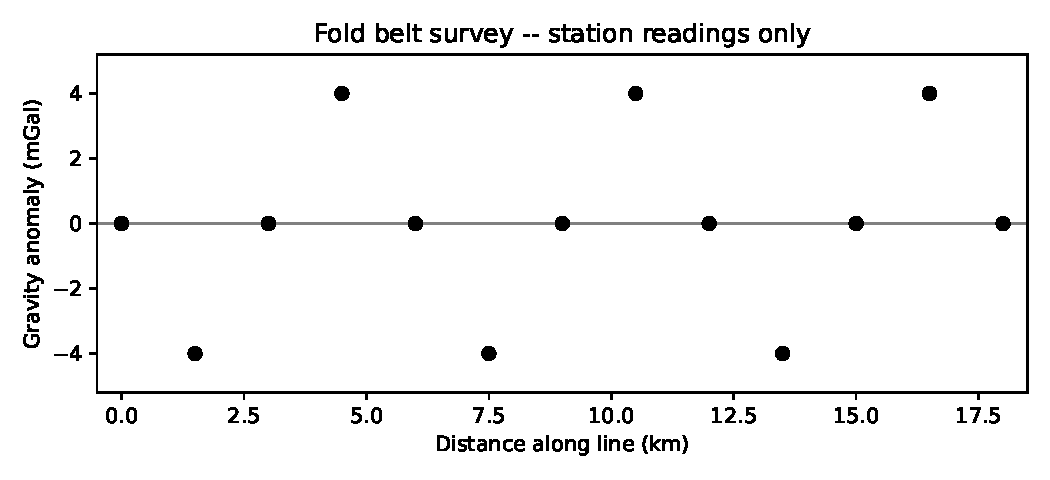
\includegraphics[width=0.85\textwidth]{figures/fig_stations_only.pdf}

            \caption{Gravity field determined from station spacing of \SI{1.5}{km}}
            \label{fig:coarse_pts}
        \end{figure}


        \item From your curve, estimate the fold wavelength (anticline-to-anticline distance).

        \answerbox[1.5cm]

        \item How many complete fold cycles does your curve show across the 18 km line?

        \answerbox[1cm]

        \item Are you confident in this interpretation? What, if anything, would make you doubt it?

        \answerbox[1.5cm]
    \end{enumerate}
\end{questions}

\textit{Do not turn the page until your instructor asks you to.}

\newpage

\begin{questions}[resume]
    \question{Phase 2 --- Six months later}
    Additional funding comes through. You return to the same \SI{18}{km} line and add \textbf{three infill stations between each of your original stations}, cutting your spacing from \SI{1.5}{km} to \SI{0.375}{km} (49 stations in total).

    \textbf{Before plotting anything}, predict:

    Do you expect the new, denser data to (a) confirm your original 6 km interpretation, (b) contradict it with a different wavelength, or (c) something else? Explain your reasoning before you plot.
    \answerbox[2.5cm]

    \begin{enumerate}[label=\roman*]
        \item Plot a smooth curve through these points. What fold wavelength do you get now?
        \begin{figure}[h]
            \centering
            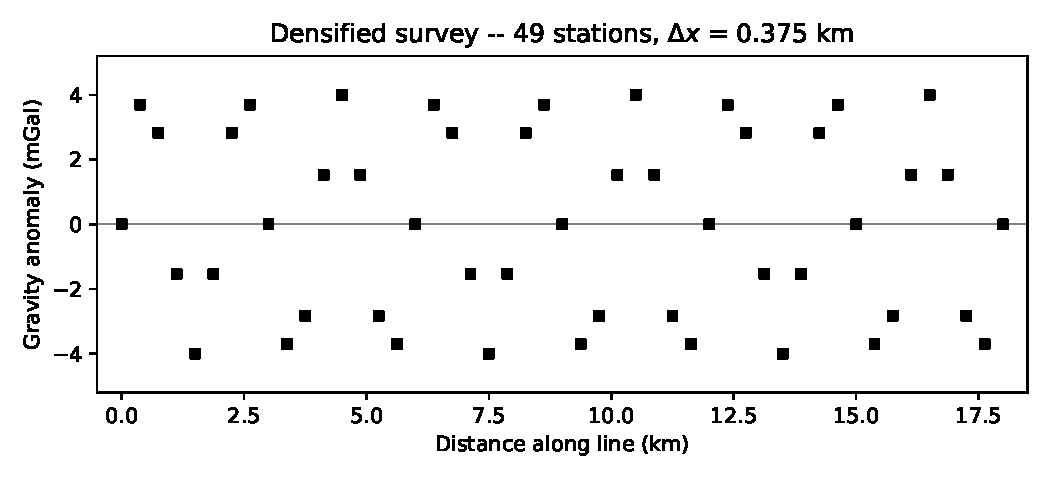
\includegraphics[width=0.85\textwidth]{figures/fig_dense_stations_only.pdf}
            \caption{Densified gravity data, now with spacing of \SI{0.375}{km}.}
            \label{fig:dense_pts}
        \end{figure}

        \answerbox[2cm]

        \item Was your prediction in Question 5 correct?
        \answerbox[1cm]
    \end{enumerate}
\end{questions}

\textit{Do not turn the page until your instructor asks you to.}

\newpage

\begin{questions}[resume]
    \question{Phase 3 --- The tension}
    Here is your densified interpretation next to your original one, together with the true structure. Original stations are circles; densified stations are squares.

    \begin{figure}[h]
        \centering
        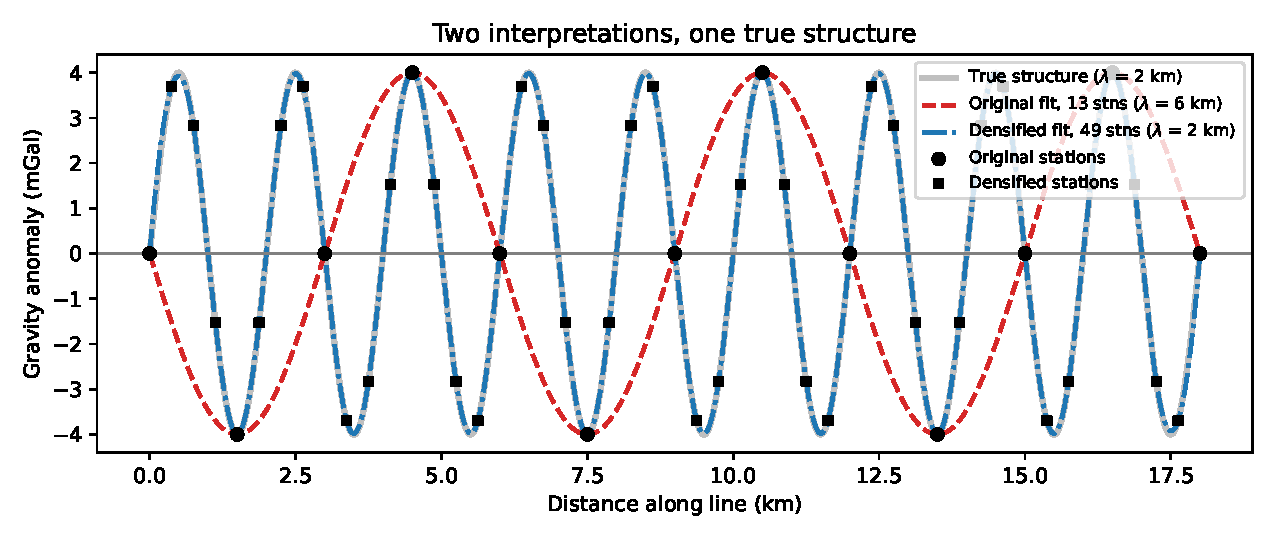
\includegraphics[width=0.85\textwidth]{figures/fig_survey_comparison.pdf}
        \caption{Comparison of smoothed gravity determined by coarse sampling (circles) and dense sampling (circles + squares).}
        \label{fig:g_compare}
    \end{figure}

    Both fitted curves pass through their own stations exactly. Neither survey was done sloppily. Yet the two surveys disagree about the fold wavelength by a factor of three.

    \begin{enumerate}[label=\roman*]
        \item Which of your two interpretations agrees with the true structure? What changed between the two surveys that made the difference --- station spacing, total number of stations, line length, or something else?
        \answerbox[2cm]

        \item \textbf{The key question:} if a third team returned and added even more infill stations between your current ones, would you expect \emph{another} new wavelength to appear, or would their result agree with what you found today? Explain your reasoning.
        \answerbox[2.5cm]

        \item Is there anything you could have noticed in the \emph{original} station data alone --- without ever densifying --- that should have made you suspicious of that first interpretation?
        \answerbox[2cm]
    \end{enumerate}
\end{questions}

\newpage

\section*{Phase 4 --- What actually happened}

This is \textbf{aliasing}: a real, higher-frequency structure disguising itself as a coherent, lower-frequency one, purely as a consequence of how often you sampled it. It is not a data quality problem and it is not fixed by more careful fieldwork at the same station spacing --- every reading you took was exact.

\subsection*{The Nyquist limit}

For a station spacing $\Delta x$, define the sampling frequency $f_s = 1/\Delta x$ (stations per km) and the \textbf{Nyquist frequency}

$$f_N = \frac{f_s}{2} = \frac{1}{2\,\Delta x}.$$

Any spatial frequency $f_{\text{true}} > f_N$ present in the real structure cannot be recovered --- it reappears (``folds back'') at an aliased frequency

$$f_{\text{alias}} = \left| f_{\text{true}} - f_s \right|, \qquad \lambda_{\text{alias}} = \frac{1}{f_{\text{alias}}}.$$

\begin{figure}[h]
    \centering
    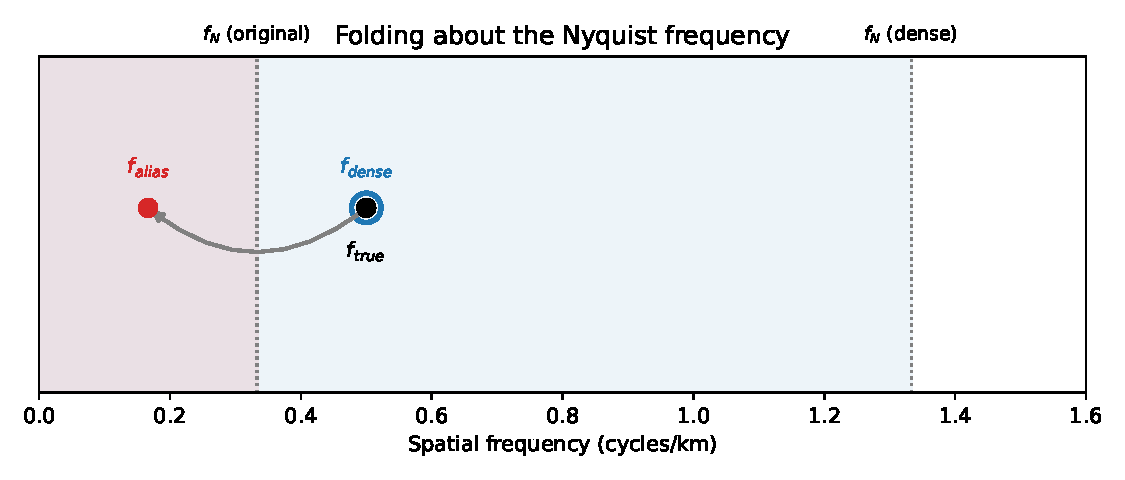
\includegraphics[width=0.85\textwidth]{figures/fig_nyquist_fold.pdf}
    \caption{Demonstration of frequency folding as a result of aliasing.  The coarse sampling results in aliasing whereas the densse sampling does not.  The Nyquist frequencies $f_{N}$ are the theoretical limits based on each survey's sampling interval.}
    \label{fig:nyquist}
\end{figure}

\subsection*{Both of your surveys, worked through}

\begin{align*}
    \text{Original: } \Delta x &= 1.5\text{ km} &\Rightarrow&& f_s &= \tfrac{1}{1.5} = 0.667\text{ cycles/km} \\
    &&&& f_N &= 0.333\text{ cycles/km} \quad (\lambda_N = 3\text{ km}) \\
    &&&& f_{\text{true}} &= \tfrac{1}{2} = 0.5\text{ cycles/km} \ (> f_N,\ \textbf{aliased}) \\
    &&&& \lambda_{\text{alias}} &= 6\text{ km} \\[2mm]
    \text{Densified: } \Delta x &= 0.375\text{ km} &\Rightarrow&& f_s &= \tfrac{1}{0.375} = 2.667\text{ cycles/km} \\
    &&&& f_N &= 1.333\text{ cycles/km} \quad (\lambda_N = 0.75\text{ km}) \\
    &&&& f_{\text{true}} &= 0.5\text{ cycles/km} \ (< f_N,\ \textbf{resolved})
\end{align*}

The true \SI{2}{km} folding was never within reach of the \SI{1.5}{km} survey ($f_{\text{true}} > f_N$, top row of the figure above) but sits comfortably inside the recoverable band once $\Delta x$ drops to \SI{0.375}{km} (bottom row) --- no folding, no ambiguity.

This answers Question 9 directly. Aliasing only happens while $f_{\text{true}} > f_N$. Once $\Delta x$ is small enough to bring $f_{\text{true}}$ under $f_N$, the true wavelength is fully recoverable, and it stays that way: adding still more stations refines the curve between existing points but cannot change which wavelength it converges to, because there is no longer any folding-back happening. A third, fourth, or hundredth team surveying this line at \SI{0.375}{km} spacing or finer would all agree with each other and with the truth. Densifying only ever produces a \emph{different} answer while you are on the wrong side of the Nyquist limit --- crossing it is a one-way trip, not an ongoing negotiation.

\subsection*{Preventing it}

The fix is decided at the survey design stage, not the interpretation stage. Recall this morning's warm-up: wavelength content is set by source depth. To resolve a structure with the shortest wavelength you expect to encounter, $\lambda_{\min}$, you need

$$\Delta x < \frac{\lambda_{\min}}{2}.$$

If you have an estimate of the shallowest source depth of interest $z_{\min}$ (from the buried-sphere relation, $\lambda \sim 1.5\,z$), this becomes a concrete field decision:

$$\Delta x \lesssim 0.75\, z_{\min}.$$

\textbf{Discussion:} for today's fold belt, what station spacing would you have needed to safely resolve \SI{2}{km} folding?

\answerbox[2.5cm]

\textbf{Key Ideas:} Aliasing produces a wrong answer that looks exactly as trustworthy as a right one. The only defence is choosing $\Delta x$ correctly \emph{before} you go to the field.

\end{activity}
